\chapter{Podwarstwa Medium Access Control}
\label{cha:mac}

Podwarstwa MAC (Medium Access Control) jest trzecią z podwarstw warstwy 2.. Z podwarstwą RLC komunikuje się ona za pośrednictwem kanałów logicznych (logical channels) i wymienia z nią jednostki danych (SDU). Natomiast z warstwą fizyczną (PHY) komunikuje się przy użyciu kanałów transportowych (transport channels) i odbiera oraz przekazuje do niej dane w formie bloków transportowych. \cite{Cox14}

\begin{figure}
	\centerline{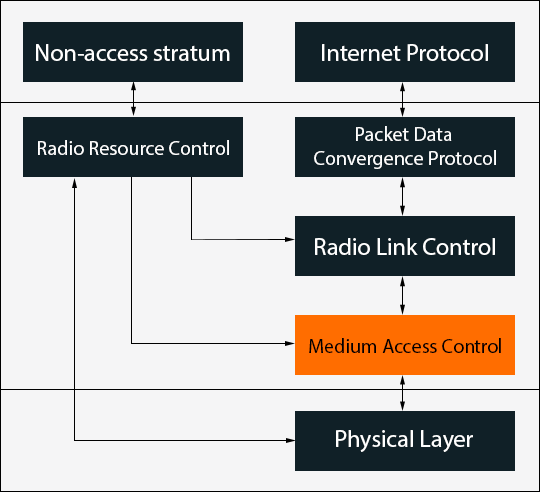
\includegraphics[width=0.4\textwidth]{images/mac_overview.png}}
	\caption{Umiejscowienie podwarstwy MAC w stosie protokołów LTE}
	\label{fig:mac_overview}
\end{figure}

Do funkcji podwarstwy MAC możemy zaliczyć:

\begin{enumerate} 
	\item Mapowanie jednostek danych (SDU) przesyłanych do kanałów logicznych na kanały transportowe gdzie formowane są w bloki tranportowe zawierające PDU
	\item Planowanie jak i kiedy jednostki danych mają zostać dostarczone
	\item Swobodny dostęp
	\item Zarządzenie synchronizacją czasu pomiędzy urządzeniem użytkownika a stacją bazową 
\end{enumerate}

\section{Mapowanie kanałów}

Podwarstwa MAC komunikuje się z podwarstwą RLC za pośrednictwem kanałów logicznych. Można je podzielić na kanały ``control channels`` transportujące dane dotyczące ``control plane`` oraz na kanały ''traffic channels'' transportujące dane dotyczące ''control plane''.

Wyróżniamy następujące kanały logiczne typu ``control channels``:

\begin{enumerate}
	\item Broadcast Control Channel (BCCH) - służy do publikowania informacji systemowych przeznaczonych do wszystkich urządzeń użytkownika w zasięgu danej stacji bazowej
	\item Paging Control Channel (PCCH) - służy do informowania urządzeń użytkownika o zdarzeniach zachodzących w sieci
	\item Common Control Channel (CCCH) - pozwala na przesyłanie informacji kontrolnych w dwóch kierunkach pomiędzy urządzeniem użytkownika i stacją bazową (dotyczy urządzeń, które nie ustanowiły połączenia na poziomie warstwy RRC)
	\item Multicast Control Channel (MCCH) - służy do publikowania informacji kontrolnych od stacji bazowej do wielu urządzeń użytkownika w ramach tzw. Multimedia Broadcast Multicast Services (MBMS)
	\item Dedicated Control Channel (DCCH) - pozwala na przesyłanie informacji kontrolnych w dwóch kierunkach pomiędzy urządzeniem użytkownika i stacją bazową (dotyczy urządzeń które ustanowiły połączenie na poziomie warstwy RRC)
\end{enumerate}

Kanały logiczne typu ``traffic channels`` są następujące:

\begin{enumerate}
	\item Dedicated Traffic Channel (DTCH) - kanał przeznaczony do transportu danych użytkownika w dwóch kierunkach pomiędzy urządzeniem użytkownika oraz stacją bazową
	\item Multicast Traffic Channel (MTCH) - słuzy do publikowania danych od stacji bazowej do wielu urządzeń użytkownika w ramach MBMS
\end{enumerate}

Z warstwą fizyczną (PHY), podwarstwa MAC komunikuje się przy użyciu kanałów transportowych ``transport channels``. Dzielimy na kanały, ktore wysyłają dane od stacji bazowej do urządzenia użytkownika tzw. ``downlink channels`` oraz kanały używane do wysyłania danych od urządzenia użytkownika do stacji bazowej ``uplink channels``.

Wyrózniamy następujące ``downlink channels``:

\begin{enumerate}
	\item Broadcast Channel (BCH) - ten kanał posiada jeden predefiniowany format przesyłania danych a także przesyła dane do wszystkich urządzeń w zasięgu danej stacji bazowej
	\item Downlink Shared Channel (DL-SCH) - wspiera korekcję błędów HARQ, dostosowywanie formatu przesyłania danych, umożliwia przesyłanie danych zarówno do pojedynczego urządzenia jak i do wielu urządzeń równocześnie, posiada wsparcie dla UE DRX w celu oszczędzania energii
	\item Paging Channel (PCH) - przesyła dane do wszystkich urządzeń w zasięgu danej stacji bazowej. Posiada wsparcia dla UE DRX, 
	\item Multicast Channel (MCH) - publikuje dane do wszystkich urządzeń w zasięgu stacji bazowej
\end{enumerate}

Oraz następujące ``uplink channels``:

\begin{enumerate}
	\item Uplink Shared Channel (UL-SCH) - oferuje wsparcie dla korekcji błędów HARQ, oferuje dynamiczne dynamiczne dostosowywanie parametrów połączenia 
	\item Random Access Channel (RACH)
\end{enumerate}

\begin{figure}
	\centerline{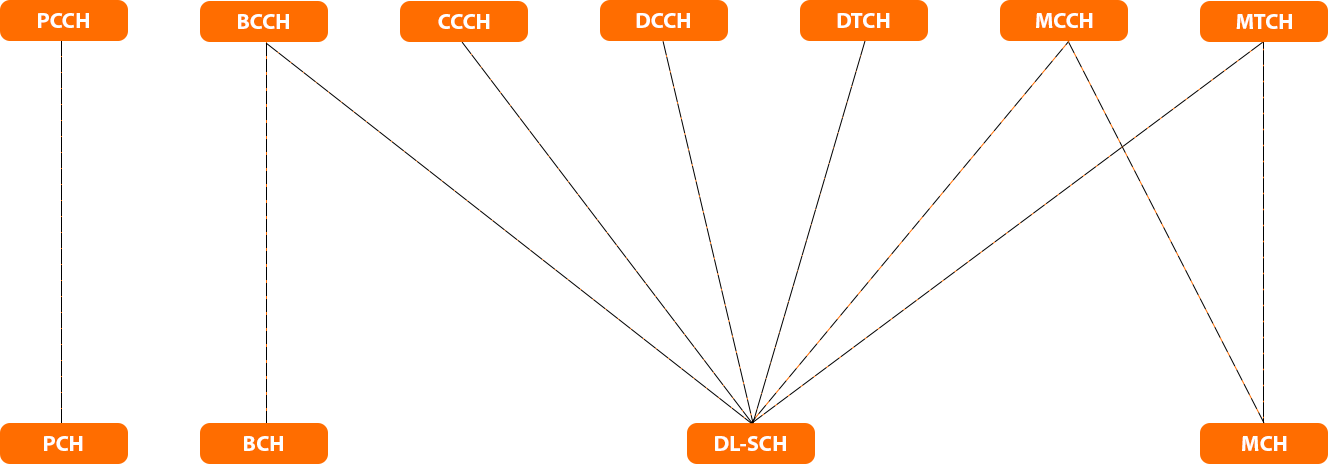
\includegraphics[width=0.8\textwidth]{images/mac_downlink_mapping.png}}
	\caption{Mapowanie kanałów logicznych na kanały transportowe dla downlink channels}
	\label{fig:mac_downlink_mapping}
\end{figure}

\begin{figure}
	\centerline{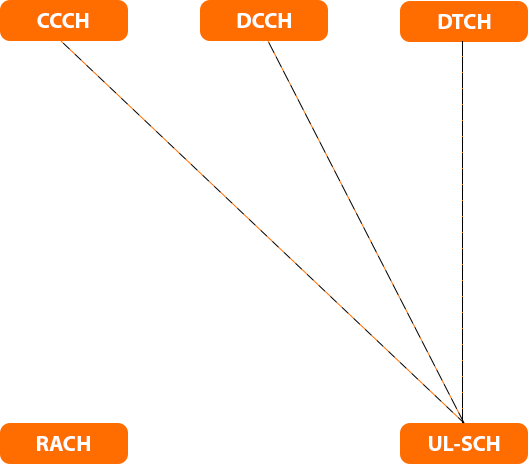
\includegraphics[width=0.5\textwidth]{images/mac_uplink_mapping.png}}
	\caption{Mapowanie kanałów logicznych na kanały transportowe dla uplink channels}
	\label{fig:mac_uplink_mapping}
\end{figure}

\section{Elementy kontrolne podwarstwy MAC}
\label{sec:mac_control_elements}

Oprócz transmisji danych użytkownika podwarstwa MAC odpowiada za wysyłanie oraz odbieranie tzw. elementów kontrolnych (MAC control elements). Wpływają one na zachowanie warstwy fizycznej. Elementy kontrolne wymieniono oraz opisano w Tabeli \ref{tab:mac_control_elements}

\begin{center}
\begin{table}
	\begin{tabular}{ | m{8em} | m{30em} | }
		\hline
		Element kontrolny & Odpowiedzialność \\
		\hline
		Buffer status report & Informacja o stanie bufora danych po stronie urządzenia użytkownika \\
		\hline
		C-RNTI & Identyfikacja urządzenia użytkownika podczas swobodnego dostępu \\
		\hline
		Power headroom & Informacja o dostępnej mocy transmisyjnej urządzenia użytkownika \\
		\hline
		Extended power headroom & Dostępna moc transmisyja podczas łączenia nośników danych \\
		\hline
		DRX command & Przełącza urządzenie użytkownika w tryb uśpienia \\
		\hline
		Timming advance command & Dostosowuje postęp czasowy w urządzeniu użytkownika \\
		\hline
		UE contention resolution identity & Rozwiązuje problem z rywalizacją o dostęp do kanału transisyjnego pomiędzy urządzeniami użytkownika podczas swobodnego dostępu \\
		\hline
		MCH scheduling information & Przesyła informacje do urządzenia użytkownika związane z planowaniem MBMS \\
		\hline
		Activation / deactivation & Aktywuje / deaktywuje dodatkowe komórki \\
		\hline
	\end{tabular}
	\caption{Elementy kontrolne podwarstwy MAC}
	\label{tab:mac_control_elements}
\end{table}
\end{center}

\section{Transmisja danych}

Aby urządzenie użytkownika mogło przesłać dane najpierw musi otrzymać od stacji bazowej slot czasowy na transmisję. Z kolei aby otrzymać slot czasowy musi poinformować stację bazową o tym, że posiada dane gotowe do wysłania. W tym celu urządzenie użytkownika wysyła element kontrolny BSR (Buffer Status Report) informujący o tym jak dużo danych jest gotowych do transmisji. BSR wysyłany jest w 3 sytuacjach:

\begin{enumerate}
	\item jeżeli po okresie gdy bufor transmisji był pusty pojawiły się w nim dane gotowe do transmisji
	\item jeżeli w buforze pojawiły się dane gotowe do transmisji o wyższym priorytecie niż dane znajdujące się do tej pory w buforze
	\item jeżeli dane w buforze oczekują na transmisje i licznik czasowy zakończył odliczanie
\end{enumerate}

W odpowiedzi na BSR urządzenie użytkownika otrzymuje od stacji bazowej informację o tym jak dużą jednostkę danych może przesłać. Nie ma tam jednak informacji o tym co taka jednostka danych może zawierać gdyż zawartość zależy od algorytmu priorytetyzacji zaimplementowanego po stronie urządzenia użytkownika.

\section{Priorytetyzacja kanałów logicznych}

Każdy z kanałów logicznych posiada przypisany priorytet od 1 do 16, gdzie mniejsza liczba oznacza wyższy priorytet. Również do każdego kanału przypisany jest parametr PBR (Prioritized Bit Rate) o wartości od 0 do 256 kbps. PBR może mieć również nieskończoną wartość, która oznacza "tak szybko jak to możliwe".

Algorytm priorytetyzacji jest następujący: w pierwszej kolejności dane są pobierane z kanałów logicznych w kolejności od kanału z najwyższym priorytetem do kanału z najniższym priorytetem. Z każdego kanału pobierana jest tylko taka ilość danych aby osiągnąć wymagany dla danego kanału bit rate. Jeżeli po przejściu przez wszystkie kanały nadal jest dostępne miejsce w wysyłanej jednostce danych, wówczas algorytm ponownie iteruje po wszystkich kanałach logicznych w kolejności od najwyższego priorytetu do najniższego i pobiera pozostałe w nich dane dopóki jednostka danych nie będzie wypełniona danymi lub dopóki wszystkie dane z kanałów logicznych nie zostaną pobrane.

\section{Korekcja błędów HARQ}

Mechanizm HARQ łączy mechanizm kontroli błędów ARQ (Automatic Repeat Request) oraz mechanizm korekcji błędów FEC (Forward Error Correction). Pozwala to uniknąć problemów związanych z korzystaniem z każdego z tych mechanizmów osobno. 
ARQ oferuje wysoką stabilność transmitowanych danych i pewność, że dotrą one bez błędów. Jednak konieczność ponawiania transmisji sprawia, że przepustowość łącza znacznie spada jeżeli występuje duża ilość błędów. A także rośnie opóźnienie w dostarczeniu danych co może mieć negatywny wpływ na usługi, które do prawidłowego działania wymagają małego opóźnienia (np. VoIP).
Z kolei FEC oferuje stałą przepustowość bez względu na liczbę błędów podczas transmisji. Minusem jest konieczność implementacji złożonych kodów do korekcji błędów, które znacznie komplikują implementację.

Mechanizm HARQ pozwala na zmniejszenie ilości ponownych transmisji danych poprzez zastosowanie mechanizmu FEC dla tego typu błędów, które występują często. Natomiast w przypadku pozostałych błędów wykonywane jest ponowna transmisja danych. Do wykrywania błędów najczęściej wykorzystywany jest mechanizm CRC.

\section{DRX}

Mechanizm DRX (Discontinuous Reception) ma za zadanie zmniejszenie zużycia baterii w urządzeniu użytkownika w okresach czasu, gdy nie bierze ono udziału w transmisji danych.

\section{Struktura pakietów}

Jednostka danych używana przy komunikacji między podwarstwą MAC a warstwą fizyczną ma ogólną strukturę przedstawioną na Rys. \ref{fig:mac_pdu}. Składa się ona z elementów kontrolnych wymienionych w sekcji \ref{sec:mac_control_elements} oraz z jednostek danych (SDU) odebranych z kanałów logicznych. Do każdego elementu kontrolnego oraz jednostki danych przypisany jest nagłówek znajdujący się w części nagłówkowej pakietu (MAC header). Nagłówki odpowiadające jednostkom danych określają ich rozmiar oraz kanał logiczny z którego pochodzą, natomiast nagłówki odpowiadające elementom kontrolnym określają ich typ oraz rozmiar. Szegółową strukturę elementu nagłówka przedstawiono na Rys. \ref{fig:mac_pdu_subheader}. Składa się on z następujących pól:

\begin{enumerate}
	\item R (1 bit) zarezerwowane pola, aktualnie nieużywane. Posiadają wartość ustawioną na 0
	\item E (1 bit) informuje czy po tym nagłówku znajdują się kolejne nagłówki. Wartość 0 oznacza, że jest to ostatnie pole nagłówka i po nim znajduje się już pierwszy element kontrolny
	\item LCID (5 bitów) dla nagłówka odnoszącego się do elementu kontrolnego zawiera on informację o typie elementu kontrolnego. Dla nagłówka odnoszącego się do jednostki danych SDU zawiera on informację o kanału logicznego z którego jednostka danych pochodzi
	\item F (1 bit) informuje o tym jaki rozmiar ma kolejne pole (Length). Wartość 0 oznacza, że pole Length ma rozmiar 7 bitów a wartość 1 oznacza, że 15 bitów
	\item Length (7 bitów lub 15 bitów) określa jaki rozmiar w bajtach ma powiązana z nagłówkiem jednostka danych (SDU)
\end{enumerate}

\begin{figure}
	\centerline{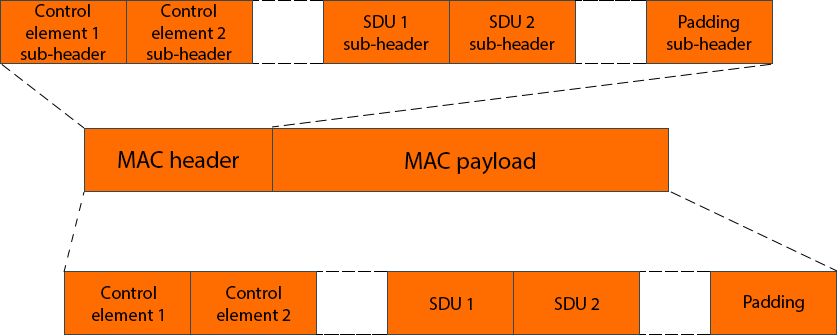
\includegraphics[width=0.8\textwidth]{images/mac_pdu.png}}
	\caption{Struktura pakietu PDU}
	\label{fig:mac_pdu}
\end{figure}

\begin{figure}
	\centerline{
\includegraphics[width=0.8\textwidth]{images/mac_pdu_subheader.png}}
	\caption{Struktura elementu nagłówka PDU}
	\label{fig:mac_pdu_subheader}
\end{figure}
